\chapter{BCS planning tool}\label{chap:tool}

\section*{}

A BCS tool, having as main objective to assist health professionals to understand the surgical outcome, requires the definition of the tumor on the specific breast of the patient. The same tool will also be used to create the dataset as explained in section \ref{sec:dataset_prep}. The tumor location and size will be used to predict the aesthetic outcome of a BCS considering the shape of the patient’s breast and the specific parameters of the tumor, using the obtained prediction models described in chapter \ref{chap:method}.

In this chapter the Functional such as Actors, Functionalities, Use cases and User stories and non Functional requirements of the software are presented, as well as some considerations concerning the interface’s design and the application flow.

\section{Functional Requirements}

The Functional requirements describes the system and its functionalities and components such as the actors and the way they interact with the system.

\subsection{Actors}

\subsubsection{Health Professional}

Both surgeons and radiologists are considered as health professional and are allowed to perform any of the functionalities presented on the tool.

\subsection{Functionalities}

The developed tool consists of the following functionalities:

\begin{itemize}
\item Loading Breast Model
\item Exporting Tumor and Excision Information, considering the breast's density
\item Visualizing model:
\begin{itemize}
\item Zoom model
\item Change model Point Size
\item Orthogonal views
\end{itemize}
\item Locating nipple
\item Breast Division:
\begin{itemize}
\item Show / hide breast's quadrants
\end{itemize}
\item Defining tumor :
\begin{itemize}
\item Tumor position, by either selecting a point or randomly choosing a position within the defined region  
\item Tumor size
\end{itemize}
\item Defining excision:
\begin{itemize}
\item Excision radius
\end{itemize}
\item Visualizing information:
\begin{itemize}
\item Tumor position - quadrant
\item Breast's Laterality
\item Breast's Volume
\item Tumor radius
\item Tumor volume
\item Excision Volume
\item Excision / Breast volume ratio
\end{itemize}
\item Undo
\item Redo
\item Reset
\end{itemize}

These functionalities will be further detailed on the use cases diagram and the user stories table.


\subsection{User Stories}

The system's user stories are described in Table \ref{tab:user stories}.

\begin{longtable}{|l|p{30mm}|l|p{90mm}|}
%\label{label}\\
\caption{User Stories of BCCT planning tool}\label{tab:user stories}\\
\hline
\textbf{ID} & \textbf{Name} & \textbf{Priority} & \textbf{Description} \\
\hline
\hline
\endhead
\hline
\endfoot
US001       & Load Model             & High                 & As a User, I want to load a specific breast's model of a patient.                    \\ \hline
US002       & Model Visualization             & High                 & As a User, I want to rotate, zoom or pan the loaded model for visualization.                   \\ \hline
US003       & Change orthogonal View             & High                 & As a User, I want to visualize the breast model on an orthogonal view (front, top, bottom, back, lateral).                    \\ \hline
US004       & Define Nipple Position             & High                 & As a User, I want to be able to define the nipple position on the point cloud.                   \\ \hline
US005       & Breast division             & Medium                 & As a User, I want to show or hide the breast quadrants (Upper Outer, Upper Inner, Lower Outer, Lower Inner).                    \\ \hline
US006       & Zoom in / Zoom out             & Medium                 & As a User, I want to Zoom in or Zoom out the breast's model.                   \\ \hline
US007       & Change point size             & Medium                 & As a User, I want to Increase or Decrease the point cloud's point size.                   \\ \hline
US008       & Define the tumor position             & High                 & As a User, I want to define the tumor's position, either by picking a point or randomly choose a point within the defined region.                  \\ \hline
US009       & Define the tumor size             & High                 & As a User, I want to define the tumor's size.                   \\ \hline
US010       & Draw the tumor sphere             & High                 & As a User, I want to see the tumor sphere drawn over the breast's point cloud.                   \\ \hline
US011       & Define the Excision radius             & High                 & As a User, I want to be able to define the margin between the excision cylinder and the tumor's radius.                    \\ \hline
US012       & Draw the Excision's cylinder             & High                 & As a User, I want to see the excision's cylinder drawn over the breast point cloud.                   \\ \hline
US013       & View the tumor quadrant             & High                 & As a User, I want to visualize in which breast's quadrant the tumor is located in.                   \\ \hline
US014       & View the breast volume             & High                 & As a User, I want to visualize the selected breast's volume.                   \\ \hline
US015       & View Tumor radius             & High                 & As a User, I want to visualize the calculated tumor radius.                   \\ \hline
US016       & View the tumor volume             & High                 & As a User, I want to visualize the tumor's volume.                    \\ \hline
US017       & View the Excised volume             & High                 & As a User, I want to visualize the volume to be excised.                   \\ \hline
US018       & View Excision/Breast volume ratio             & Medium                 & As a User, I want to see the percentage of the breast volume to be excised.                    \\ \hline
US019       & Export excision and tumor point cloud information             & High                 & As a User, I want to record the model points that were considered the tumor or the excision portion.                   \\ \hline
US020       & Reset             & Medium                 & As a User, I want to restore the state of the system, re-loading the breasts' models to their initial state.                   \\ \hline
US021       & Undo             & Medium                 & As a User, I want to restore the system to the previously state, ignoring the last step.                    \\ \hline
US022       & Redo             & Medium                 & As a User, I want to perform the previously undone step.                   \\ \hline
US023       & Hide the tumor sphere             & Medium                 & As a User, I want to hide the tumor sphere previously drawn.                   \\ \hline
US024       & Hide the excision cylinder             & Medium                 & As a User, I want to hide the excised cylinder previously drawn.                   \\ \hline

\end{longtable}

\subsection{Use cases}

Figure \ref{fig:use_cases} describes the possible interactions that a user can have in the tool. Note that simple interactions were ignored.

\begin{figure}[!h]
\begin{center}
    \leavevmode
    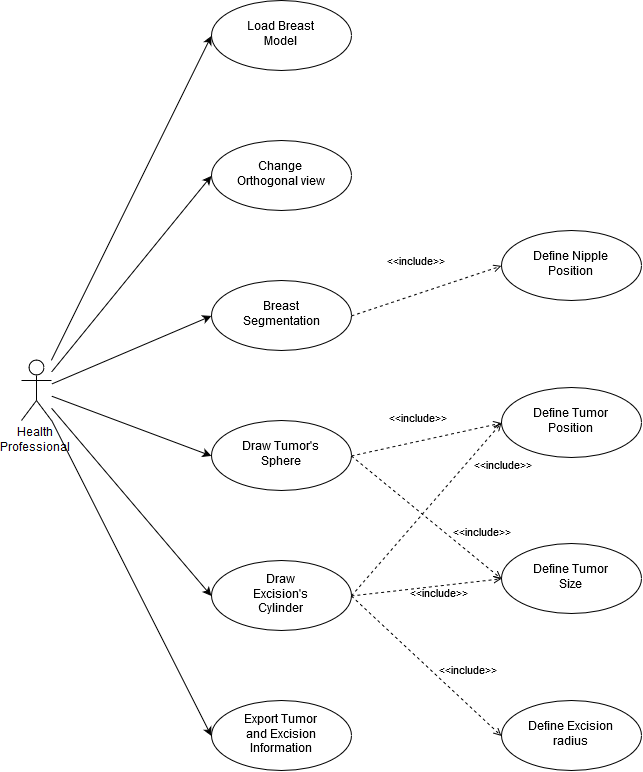
\includegraphics[width=0.7\textwidth]{Use_Cases}
    \caption[BCS planning tool Use Cases]{Use cases for the BCS planning tool}
    \label{fig:use_cases}
  \end{center}
\end{figure}

\subsection{Functional Constraints}

The developed tool have some constraints, due to the representation of the breast model as a point cloud. Those constraints are presented below:
\begin{itemize}
\item When selecting both the nipple and tumor position, must be a point from the model's point cloud;
\item The calculation of the breast, tumor and excision volumes are calculated through approximations;
\item When defining the tumor's sphere and the excision's cylinder, the breast boundaries are not taken into account. This way, the defined polygon will be drawn disregarding the point clouds' limits.
\end{itemize}

\section{Non Functional Requirements}

These are the requirements that are not crucial for the normal function of the application but enhance the user's experience. 

\begin{itemize}
\item \textbf{Interface:} The user interface must be intuitive allowing the user to access all the functionalities with the minimal interaction with the tool in a logical way. To enhance this process many of the functionalities despite of being always visible are only enable when the system has enough information to perform it. In some cases the system warns the user to add necessary information before performing the task;
\item \textbf{Maintenance:} The tool was developed in a way to easily modify the implemented functionalities of the system;
\item \textbf{Expandability:} The tool was developed in a way to easily extend or add additional functionalities to the system;
\item \textbf{Efficiency:} The tool performs all the system's function on a short time.
\end{itemize}


\section{Application Flow}

The flow presented in Figure \ref{fig:tool_flow} shows the required steps to perform the BCS planning. All the tasks not presented on the flow are done at any moment after loading the breast's model.

\begin{figure}[!h]
\begin{center}
    \leavevmode
    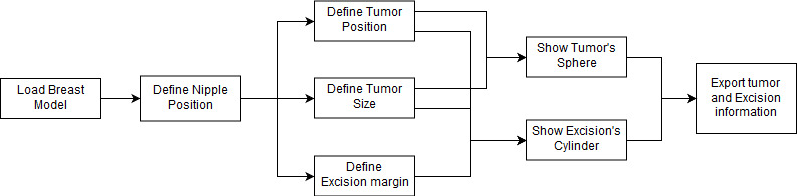
\includegraphics[width=1.0\textwidth]{tool_flow_2}
    \caption[BCS planning tool flow]{Tool flow with the required steps to perform the BCS planning}
    \label{fig:tool_flow}
  \end{center}
\end{figure}

\section{Development}

The frameworks used for the development of the described application are explained below and were implemented using C++. A few frameworks such as Qt and VTK were also used in order to simplify the tool's interface development.

\subsection{System Documentation}
All the developed codes were written clearly and in a straightforward way in order to allow a intuitive and fast reading of each function and described object.

\subsection{C++}
All the required functions where declared on the header files and respectively implemented on the correspondent \textit{cpp} file. Besides the utilization of this types of file, there is a main file responsable for the execution of the interface and all the functions associated with it, and a \textit{ui} (user interface) file where the interface was designed.

\subsubsection{Code comments}
The code comments, as a way of code documentation, are only used when necessary decreasing the amount of visual barriers, often associated with mathematical formulas or required calculations on the 3D space.

\subsection{Used Frameworks}

\subsubsection{Qt}

Qt allows the development of multi-platform applications and interfaces based on C++ in a simple and fast way \footnote{\url{http://doc.qt.io/}}.

\subsubsection{VTK}
The Visualization Toolkit (VTK) is an open-source software system used for 3D computer graphics, image processing, and visualization that consists of a C++ class library including several interpreted interface layers \footnote{\url{http://www.vtk.org/documentation/}}. VTK integrates other frameworks such as Qt, also used for the development of this application.

\subsubsection{Boost library}
Boost library is a C++ set of libraries that allows an easy utilization of linear algebra, image processing and multithreading. These libraries are required for the utilization of VTK and Qt frameworks.

\section{Interface}

Figure \ref{fig:tool_interface} shows the interface of the main functionalities of the tool. When launching the tool, the initial window will be displayed, where it is only possible to load a breast's point cloud \subref{fig:initial_view}. After loading the breast's model, the nipple's position feature is enabled. The breast's point cloud is also displayed on the visualization area. A selection point view for the nipple position is presented in \subref{fig:point_selection}. For the tumor position a similar view will be displayed with the breast seen from a frontal position. After defining the nipple position, the breast can be divided into quadrants. This can be seen through planes drawn over the breast in \subref{fig:segmentation_view}. In order to do the tumor definition, tumor position is selected as well as a tumor size. If one of the fields is not checked, a warning window will be displayed \subref{fig:warning_alert}. When all the fields are completed, a tumor's sphere can be drawn and displayed over the breast on the visualization area \subref{fig:tumor_view}. Last, but not least, when selecting an excision margin, the excision's cylinder is drawn \subref{fig:excision_view}.

Regarding the interface, this was created considering the target group and adapted according to its propose. One of the aspects that were took into consideration was the used icons. Due to the lack of materials guidelines and icons to represent some of the intended actions, some icons used in the tool were created in order to overcome that lack and the ones that already existed were adjusted to provide an overall consistency among all the tool. Other human-computer iteration principles were considered as the representation of already clicked buttons, and the pop-up of warning and dialog messages to inform the user about any error or task completion. The tool's interface is displayed in Figure \ref{fig:loaded_r}, where the interaction panels are delimited and coupled with a label.

\begin{figure}[!h]
\centering
\scalebox{1.1}{%
\begin{tabular}{ll}
\subfloat[Initial view]{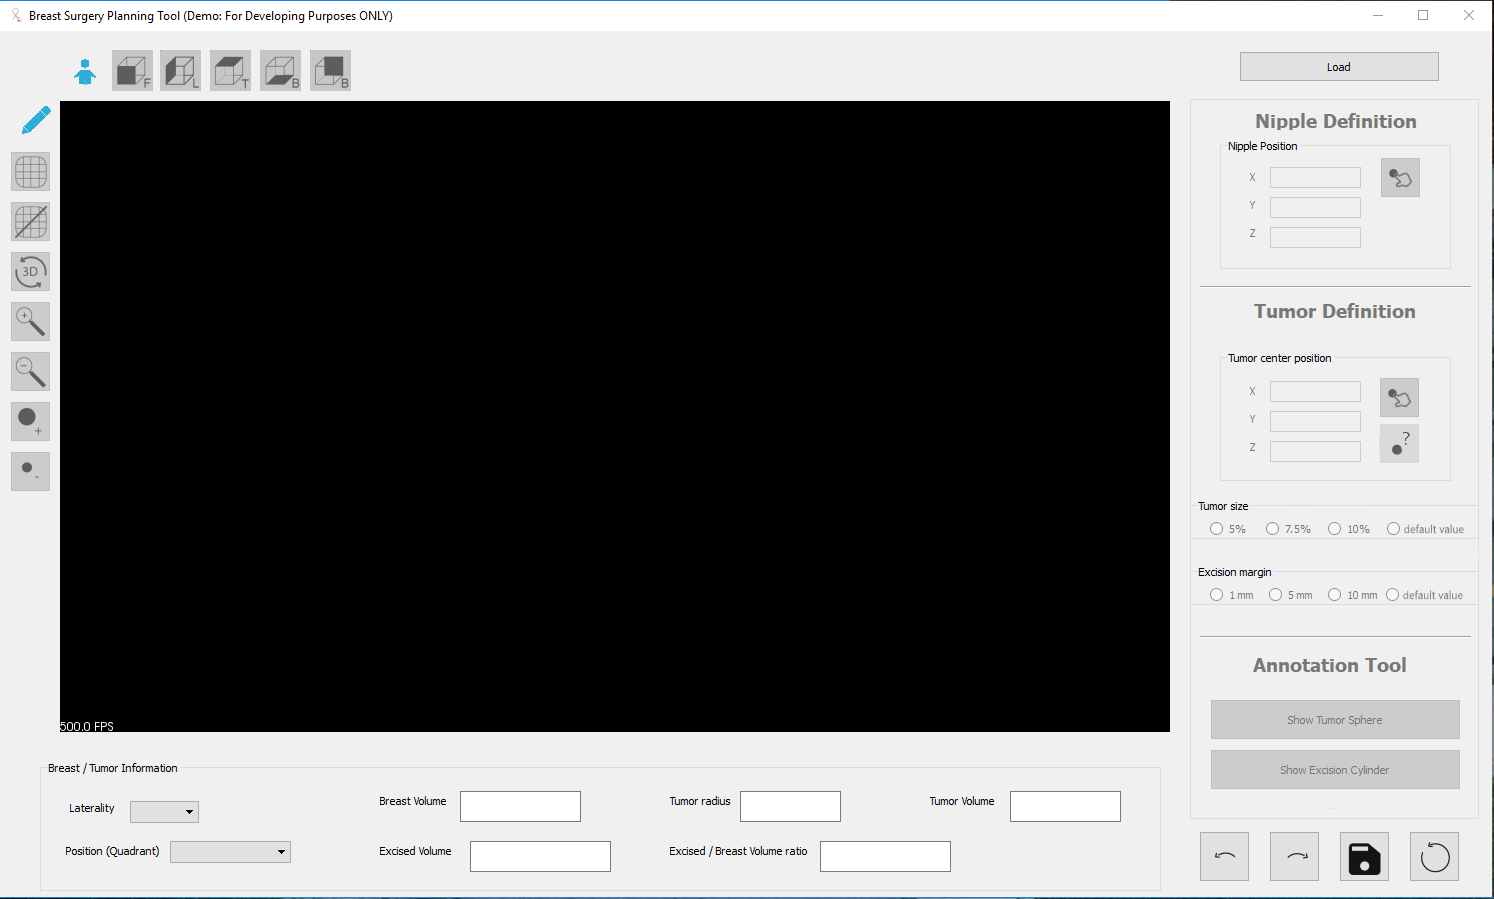
\includegraphics[width = 3in]{initial_r2}\label{fig:initial_view}} &
\subfloat[Point Selection View]{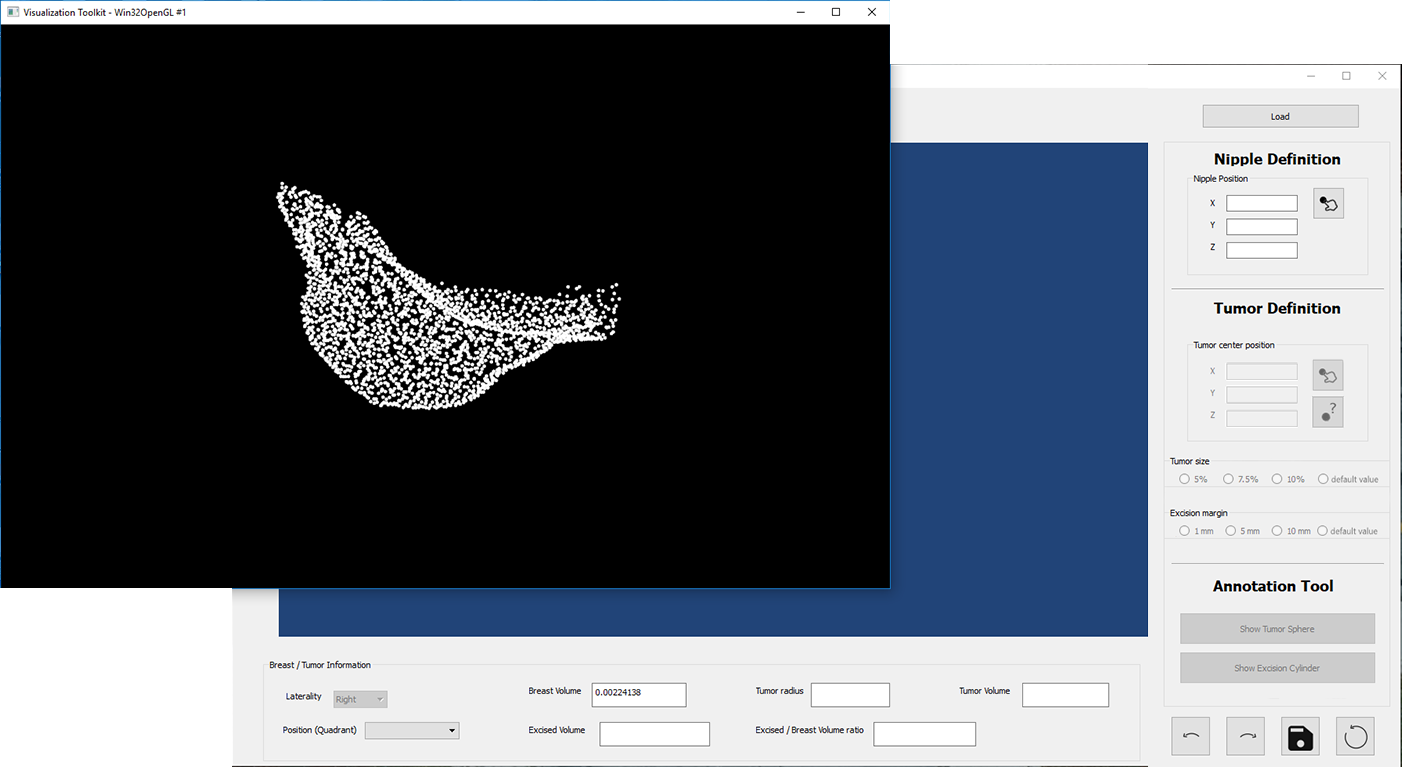
\includegraphics[width = 3in]{point_selection_r2}\label{fig:point_selection}}\\
\subfloat[Breast Segmentation View]{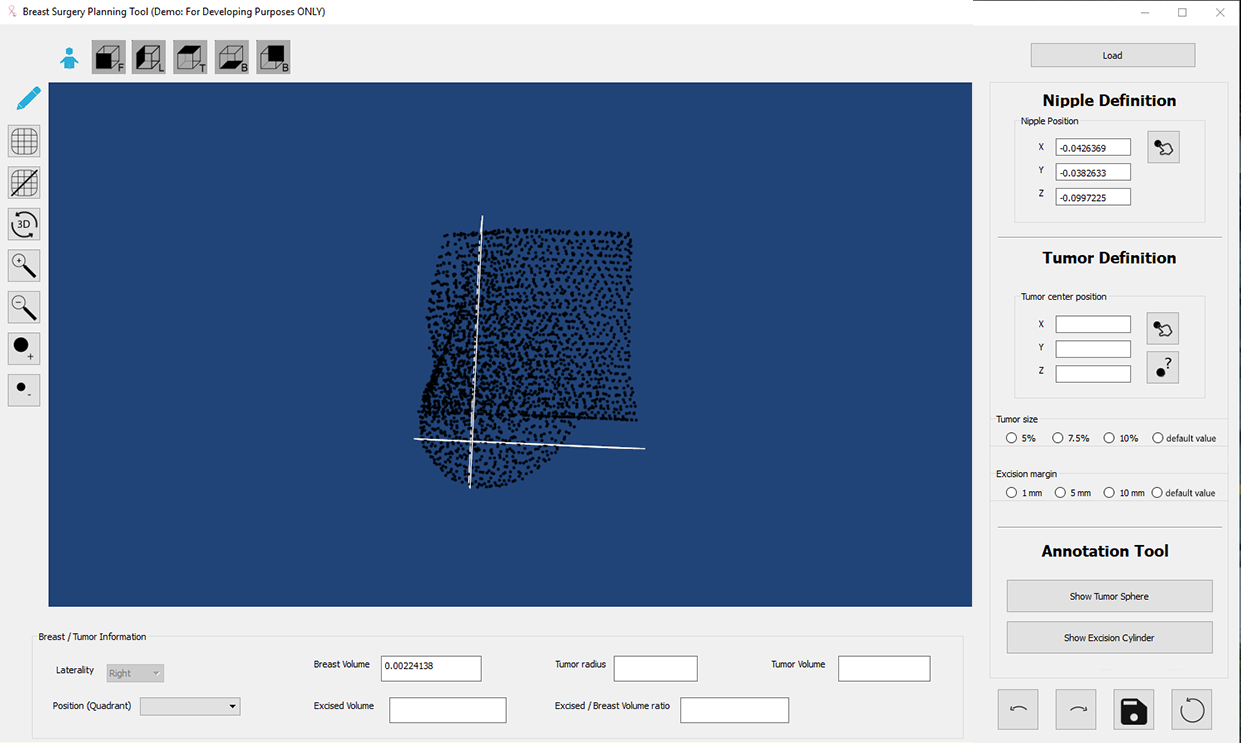
\includegraphics[width = 3in]{segmentation_r2}\label{fig:segmentation_view}} &
\subfloat[Warning Alert]{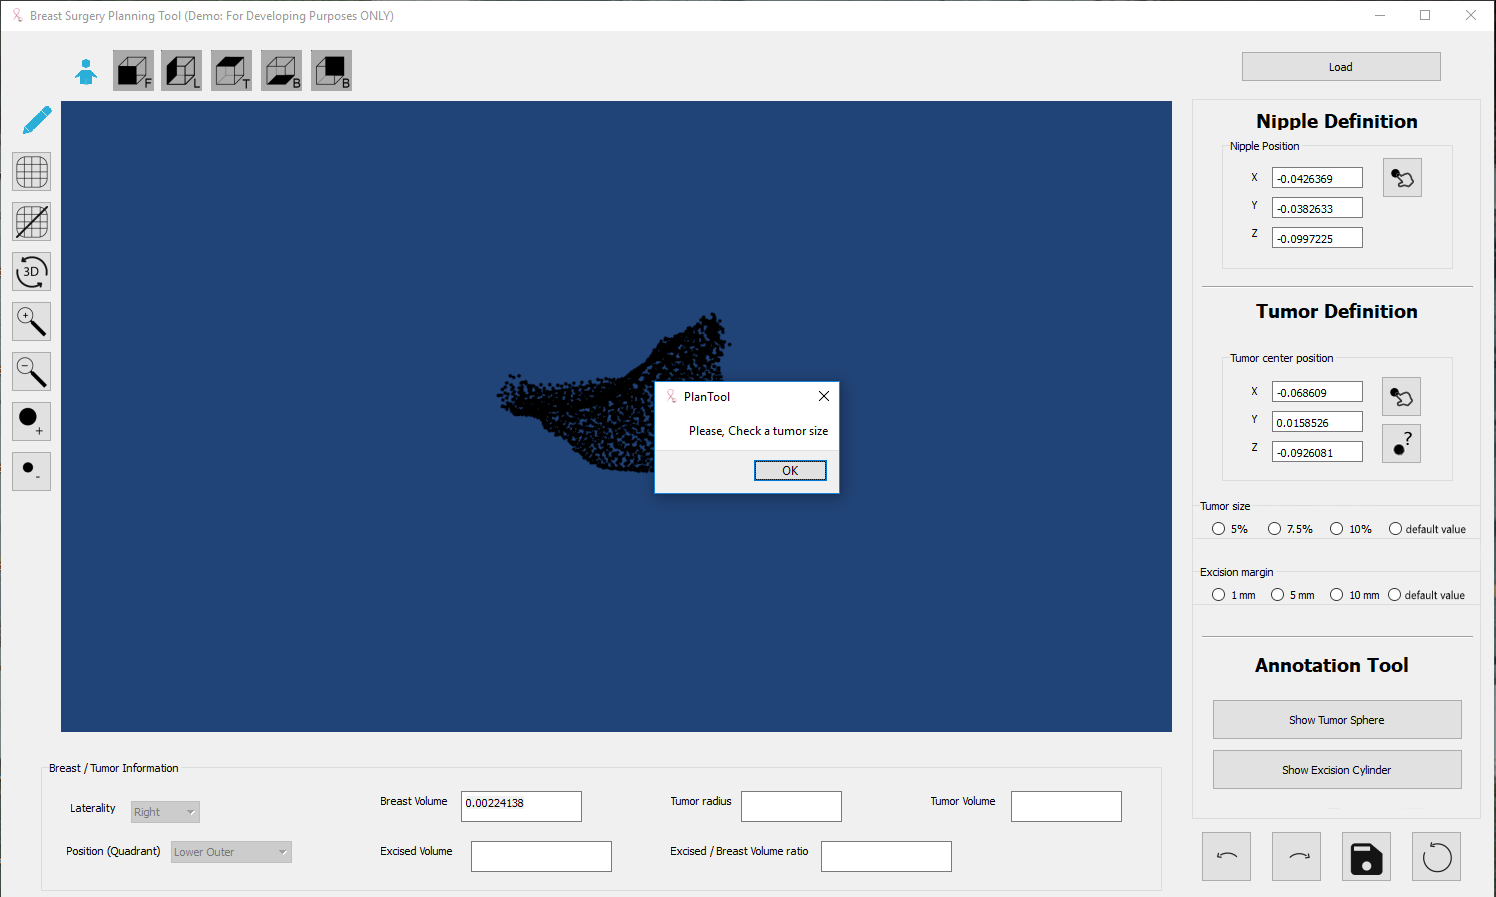
\includegraphics[width = 3in]{warning_r2}\label{fig:warning_alert}}\\
\subfloat[Tumor's view]{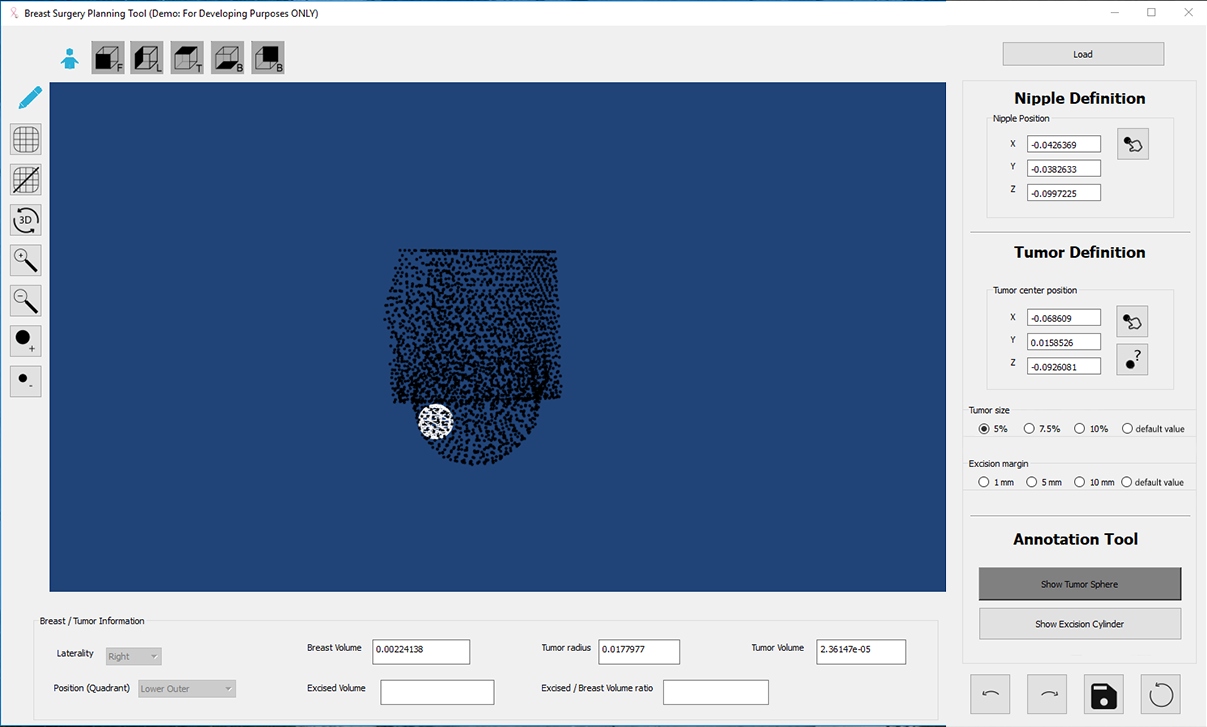
\includegraphics[width= 3in]{tumor_def_r2}\label{fig:tumor_view}} &
\subfloat[Excision's view]{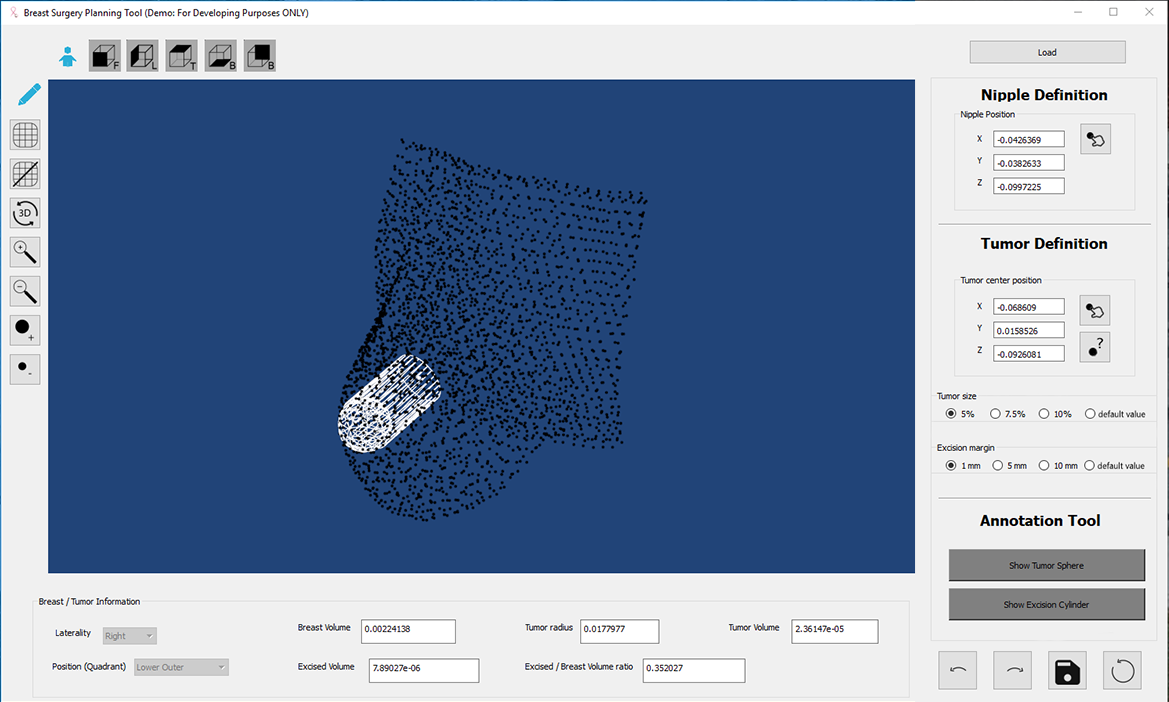
\includegraphics[width = 3in]{cylinder_def_r2}\label{fig:excision_view}} \\
\end{tabular}
}
\caption[BCS planning tool interface]{Interface of several views of the BCS planning tool}
\label{fig:tool_interface}
\end{figure}

\begin{figure}[!h]
\centering
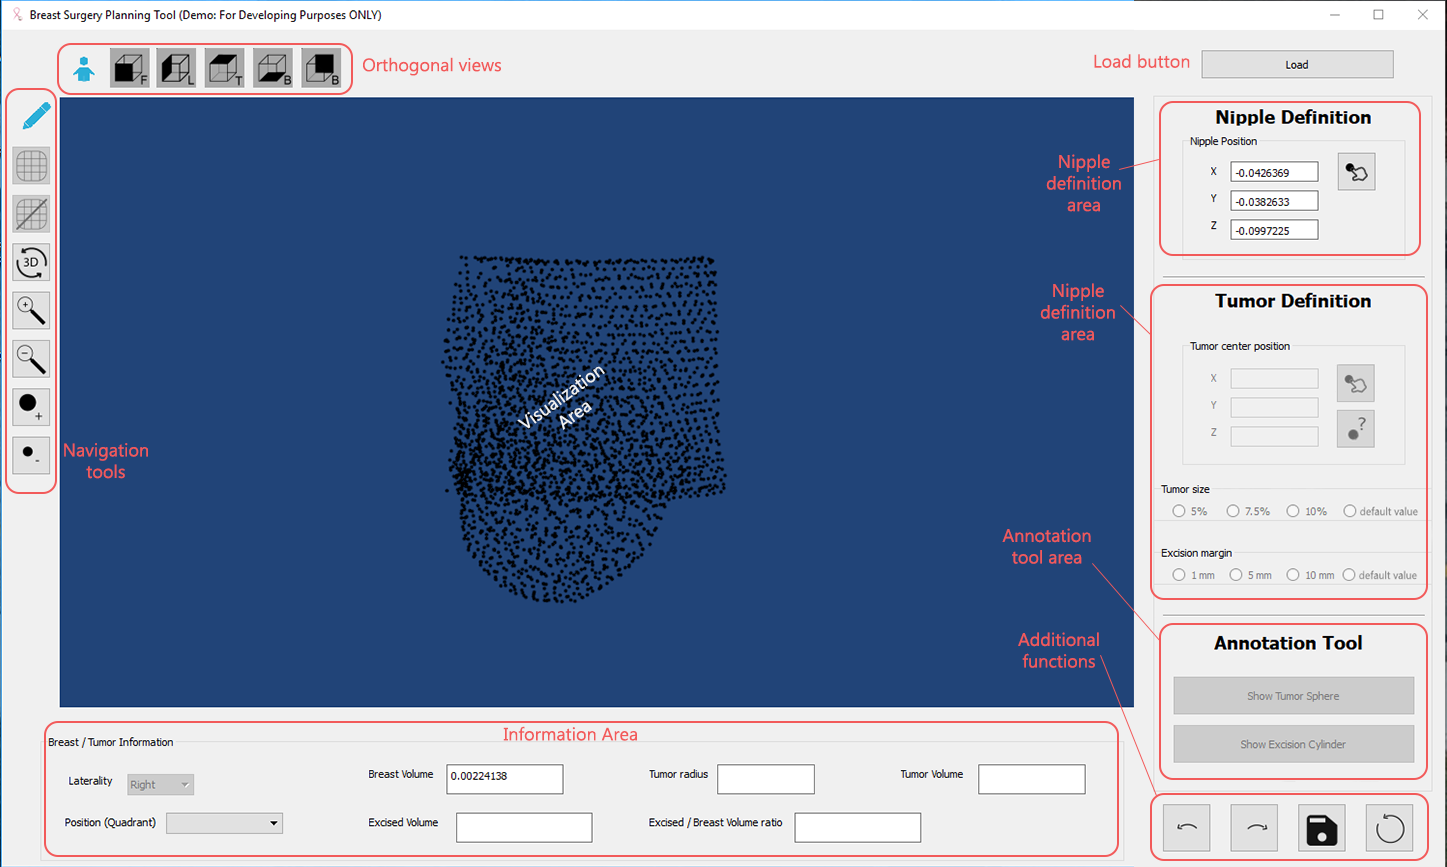
\includegraphics[width=1.0\textwidth]{loaded_r2}
    \caption[BCS planning Tool Interface]{BCS Tool Interface}
    \label{fig:loaded_r}
\end{figure}


\section{Summary}
In this chapter the developed BCS planing tool was presented as well as both functional and non functional requirements, application flow, the frameworks that were used. Also some considerations regarding its development and implementation are described as well as some interfaces of the application.

One of the most valuable functionalities that the tool can be equipped with is to allow the simulation and further visualization of the breast's deformations predicted by the models described in chapter \ref{chap:method}.